\section{Symulacje układów}
    Podczas symulacji sprawdzono działanie kilku bloków funkcjonalnych, tj. PSU, sumator, generator szumu białego oraz 
    wzmacniacz pomiarowy. Symulacja czasowa PSU pozwoliła sprawdzić jak duży będzie przerzut napięcia podczas uruchomiania 
    układu. Wyniki przedstawiono na rysunku \ref{fig:sym_LM1117}.  
    Jako sumator postanowiono skorzystać ze schematu z noty AN5537 od ST Microelectronics. Symulacja potwierdziła 
    wcześniejsze przypuszczenia - układ zasilany niesymetrycznie nie toleruje napięć ujemnych. W związku z tym 
    iteracyjnie naniesiono potrzebne poprawki, by układ mógł pracować bez zniekształceń z szumem o zerowej składowej stałej. 
    Wyniki symulacji przedstawia rysunek \ref{fig:sym_sum}. 
    \begin{figure}[!ht]
        \centering
        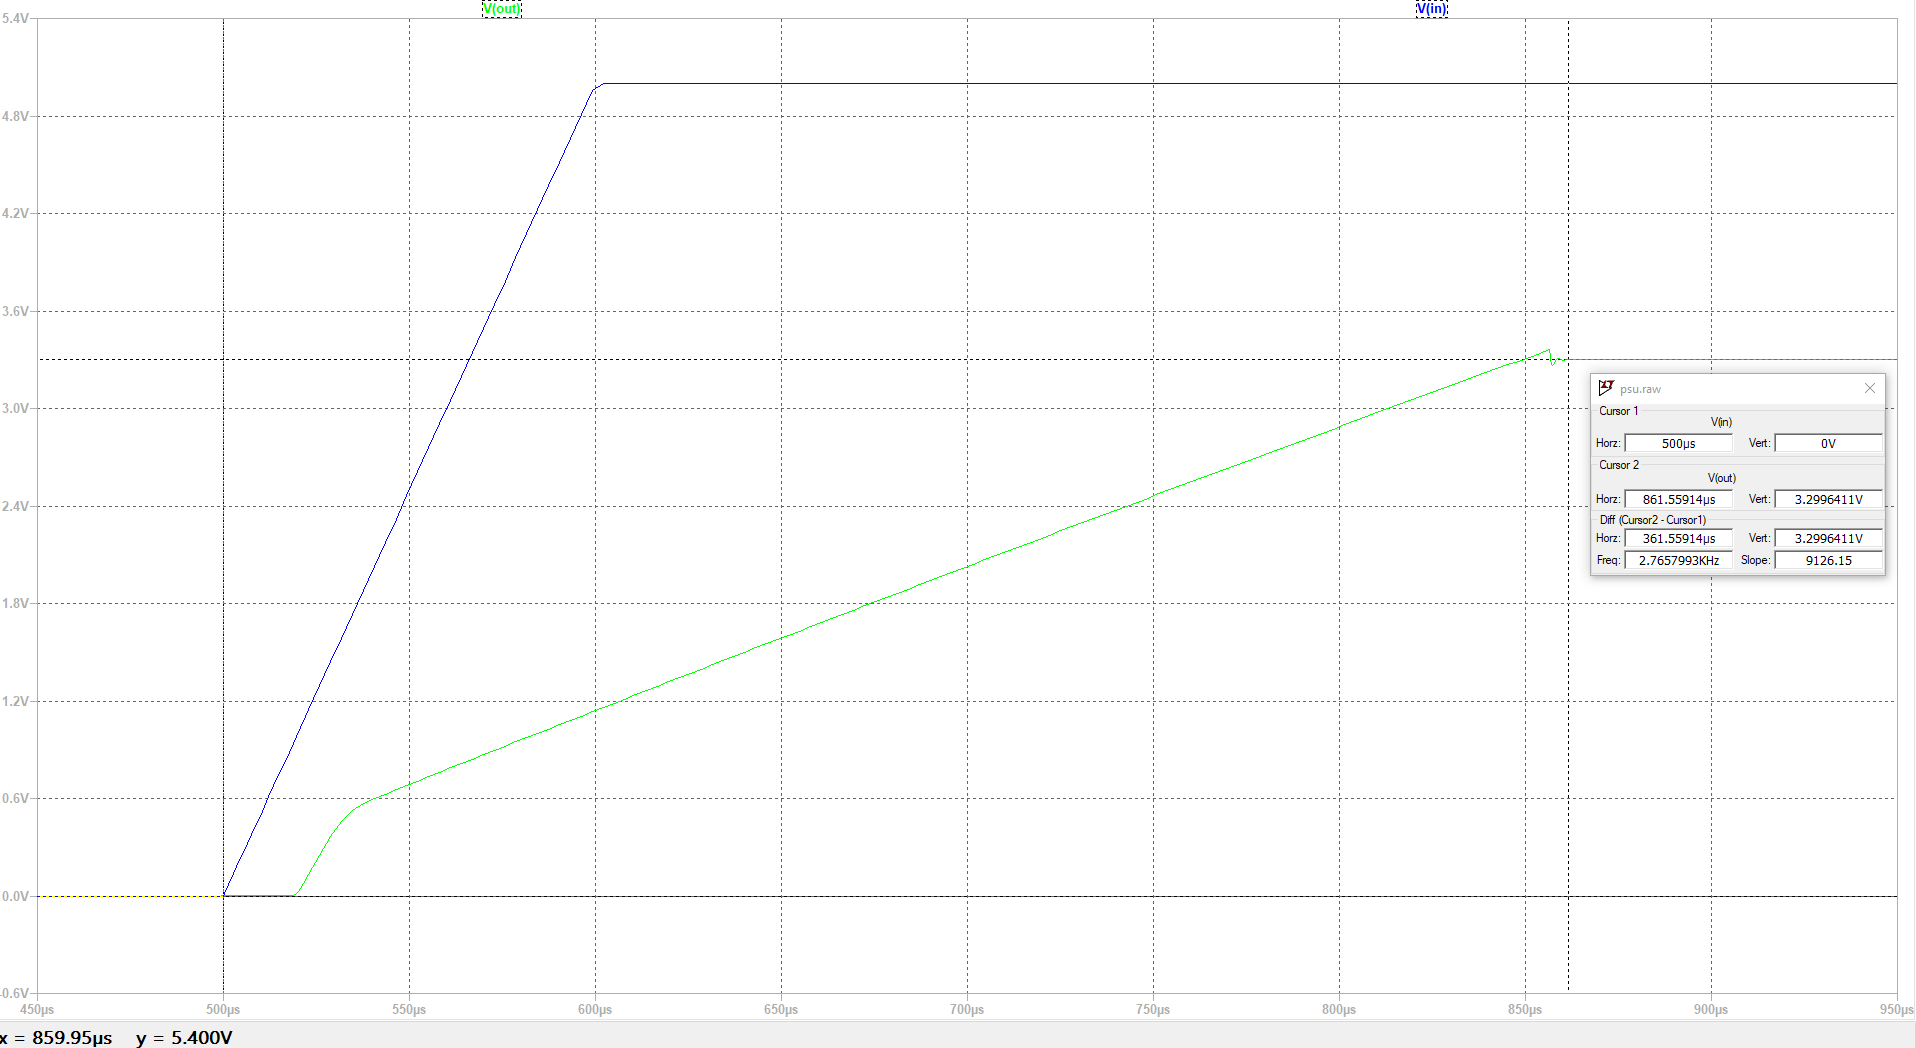
\includegraphics[width=\textwidth]{psu_tran.png}
        \caption{Symulacja tran stabilizatora napięcia LM1117-3.3 napięcia wejściowego ($V_{in}$) i wyjściowego ($V_{out}$).}
        \label{fig:sym_LM1117}
    \end{figure}
    \begin{figure}[!ht]
        \centering
        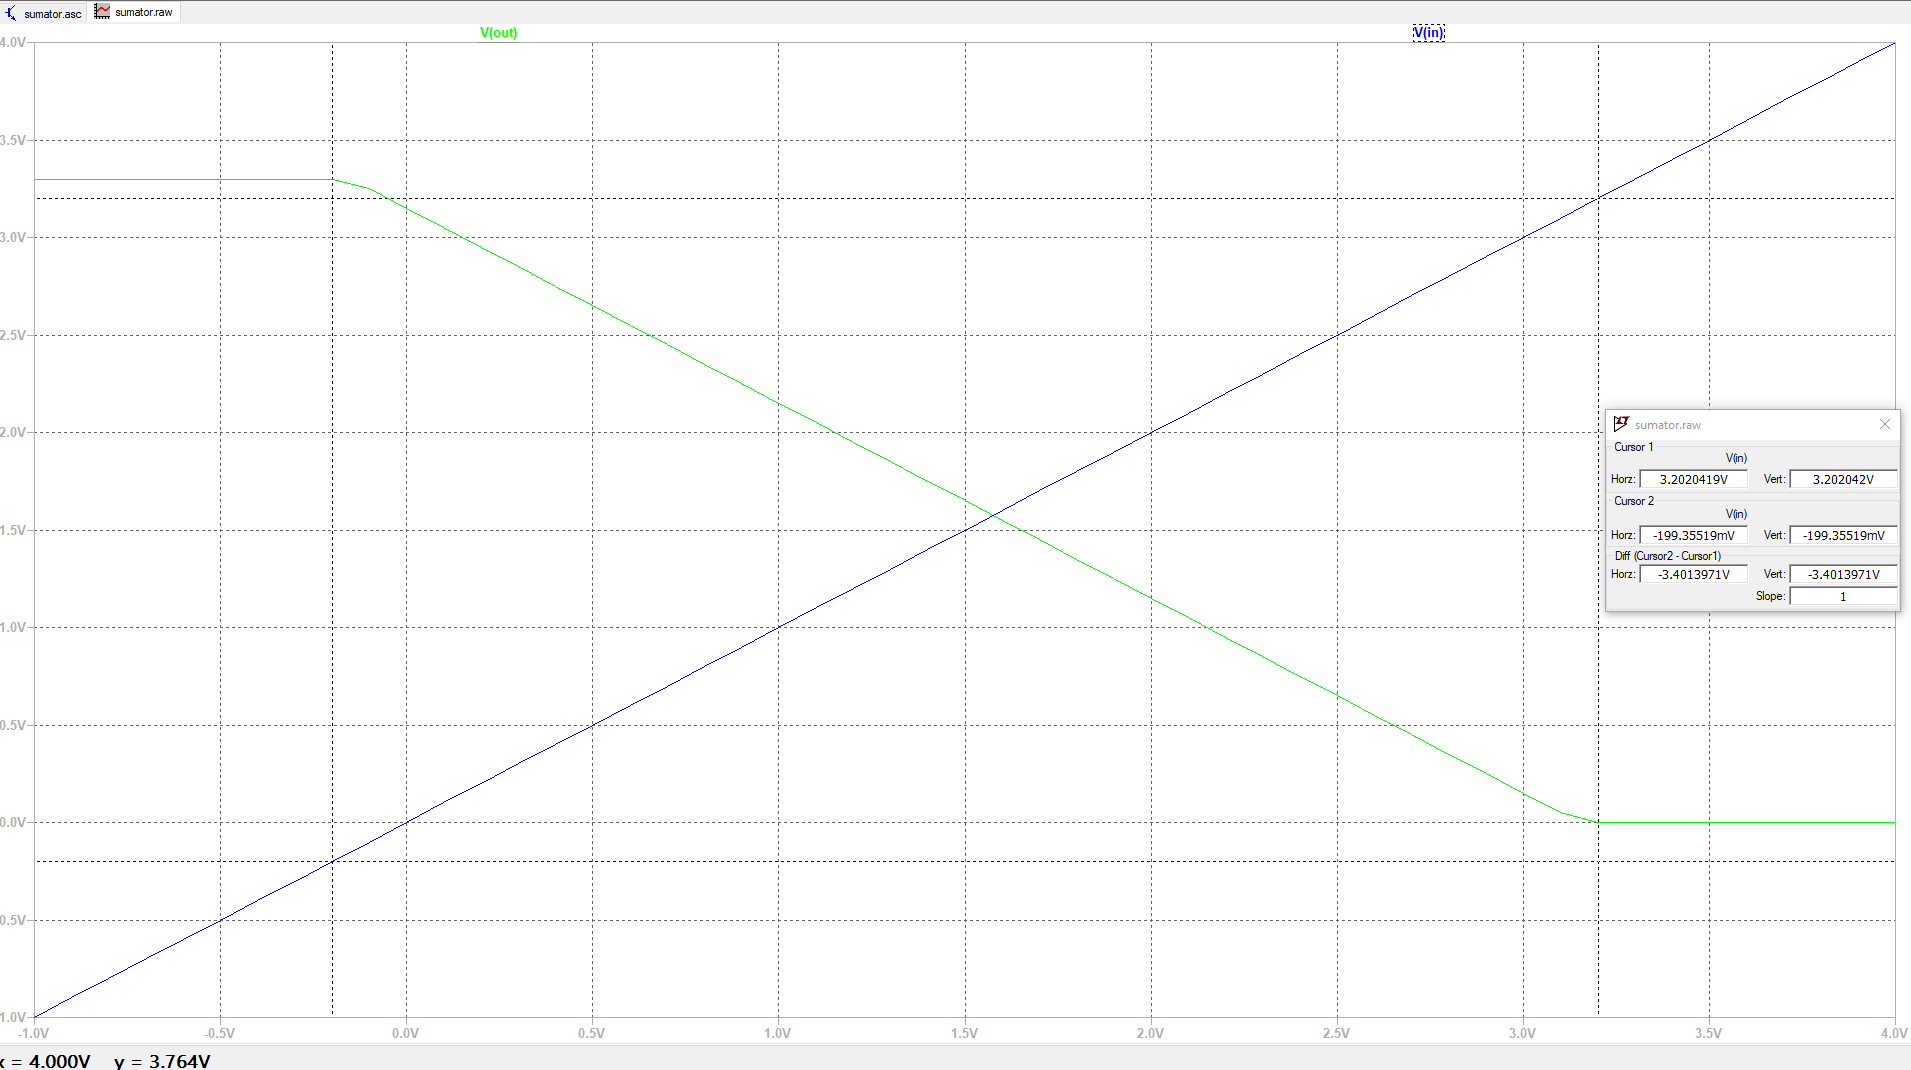
\includegraphics[width=\textwidth]{sumator_dc.png}
        \caption{Symulacja dc układu sumującego, napięcia wyjściowego ($V_{out}$) od napięcia wejściowego ($V_{in}$).}
        \label{fig:sym_sum}
    \end{figure}
    
    Podczas symulacji wzmacniacza pomiarowego okazało się, że możliwe będzie zmierzenie prądów o natężeniu $1\ nA$. Czułość 
    wzmacniacza określono na $\frac{1\ mV}{1\ nA}$. Zakres pomiarowy wynosi $\pm 1\ \mu A$, a dopuszczalny zakres napięcia 
    wspólnego, przy maksymalnym prądzie wynosi $\approx 0.7\ V \div \approx 2.8\ V$. Zależność napięcia wyjściowego 
    od prądu wejściowego przedstawiono na wykresach \ref{fig:sym_INA_100n} i \ref{fig:sym_INA_1u}. 
    Zależność napięcia wyjściowego od wejściowego napięcia wspólnego dla prądu $1\ \mu A$ została przedstawiona na wykresach 
    \ref{fig:sym_INA_CM} i \ref{fig:sym_INA_CM_follower}. Schemat symulacyjny przedstawiono na rysunku \ref{fig:sym_CM_sch}.
    \begin{figure}[!ht]
        \centering
        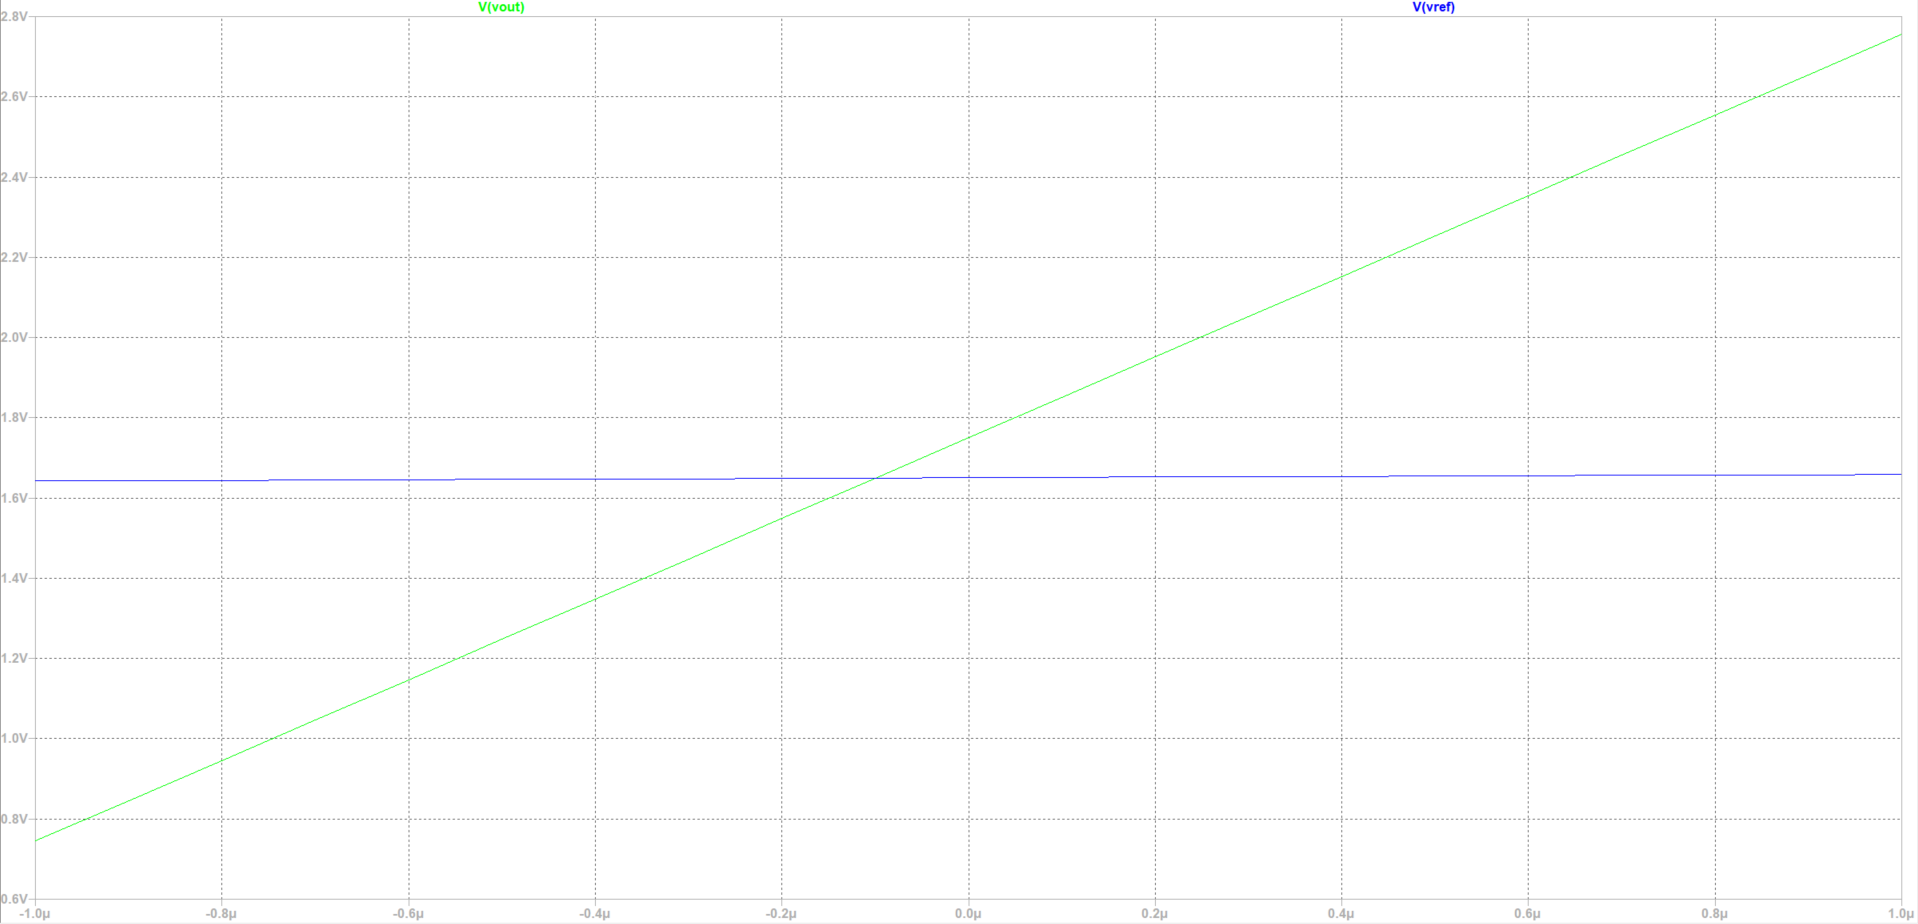
\includegraphics[width=\textwidth]{INA333_1u_range.png}
        \caption{Symulacja parametryczna wzmacniacza pomiarowego w zakresie $\pm 1\ \mu A$.}
        \label{fig:sym_INA_1u}
    \end{figure}
    \begin{figure}[!ht]
        \centering
        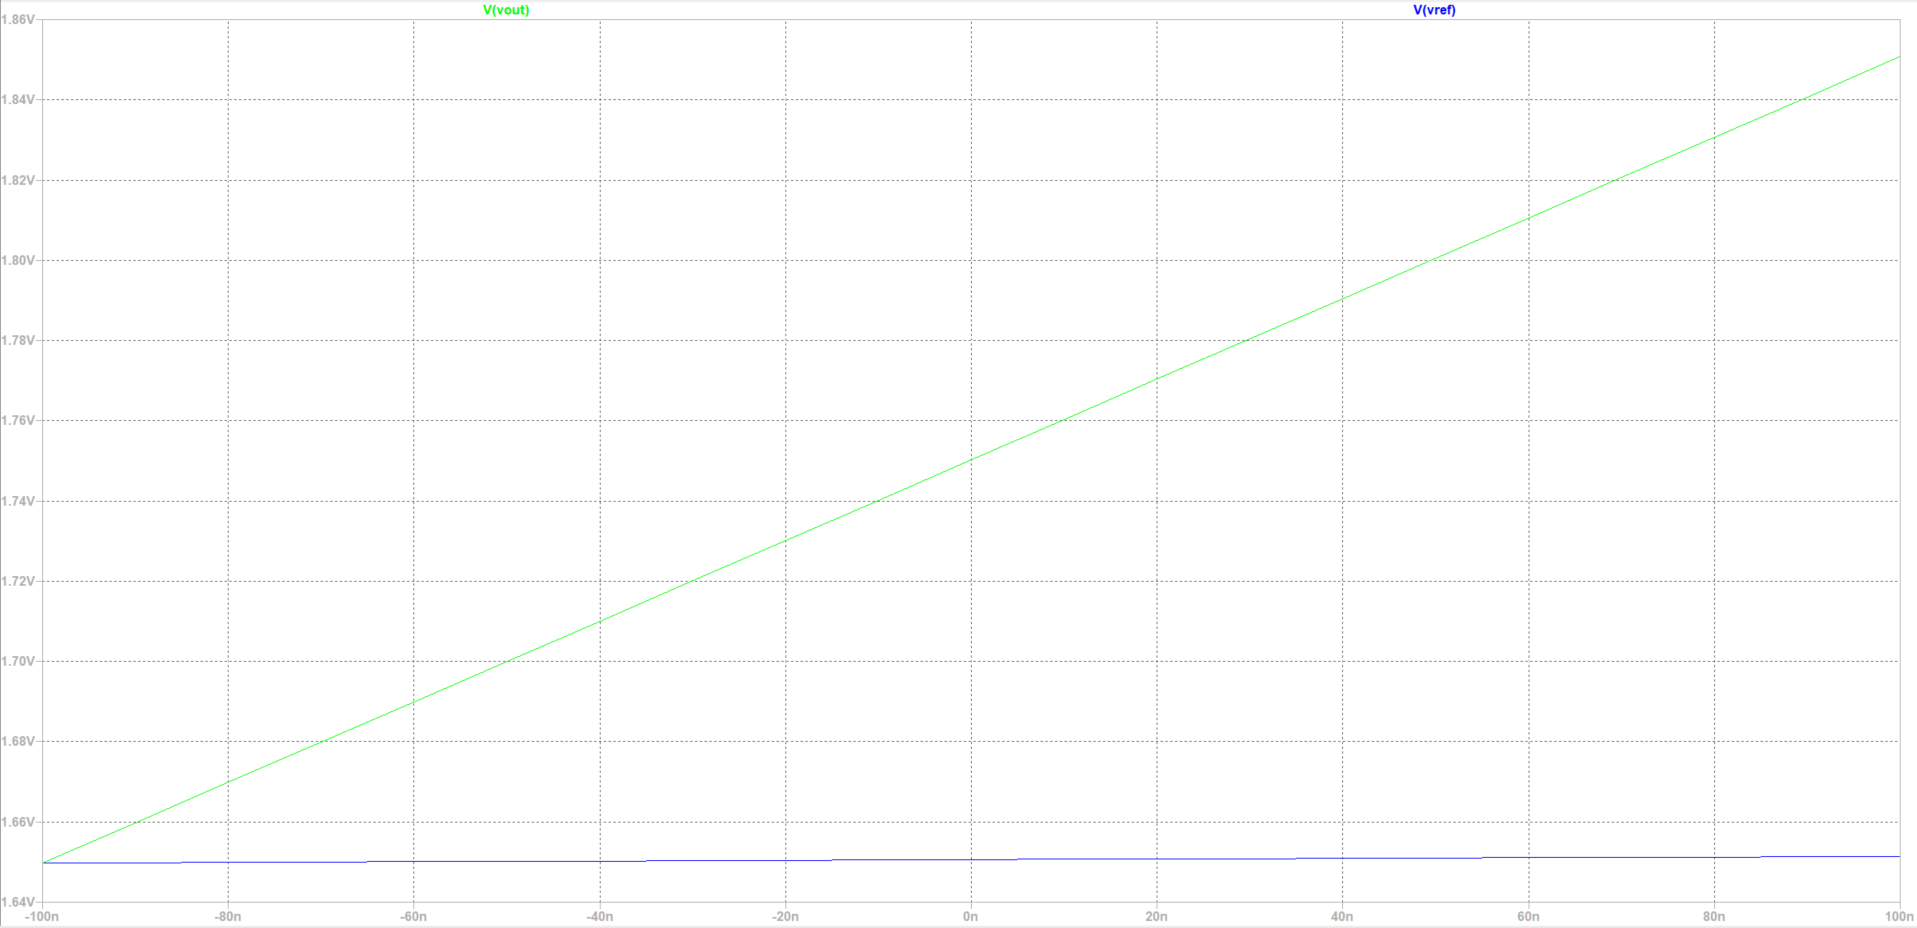
\includegraphics[width=\textwidth]{INA333_100n_range.png}
        \caption{Symulacja parametryczna wzmacniacza pomiarowego w zakresie $\pm 100\ nA$.}
        \label{fig:sym_INA_100n}
    \end{figure}
    \begin{figure}[!ht]
        \centering
        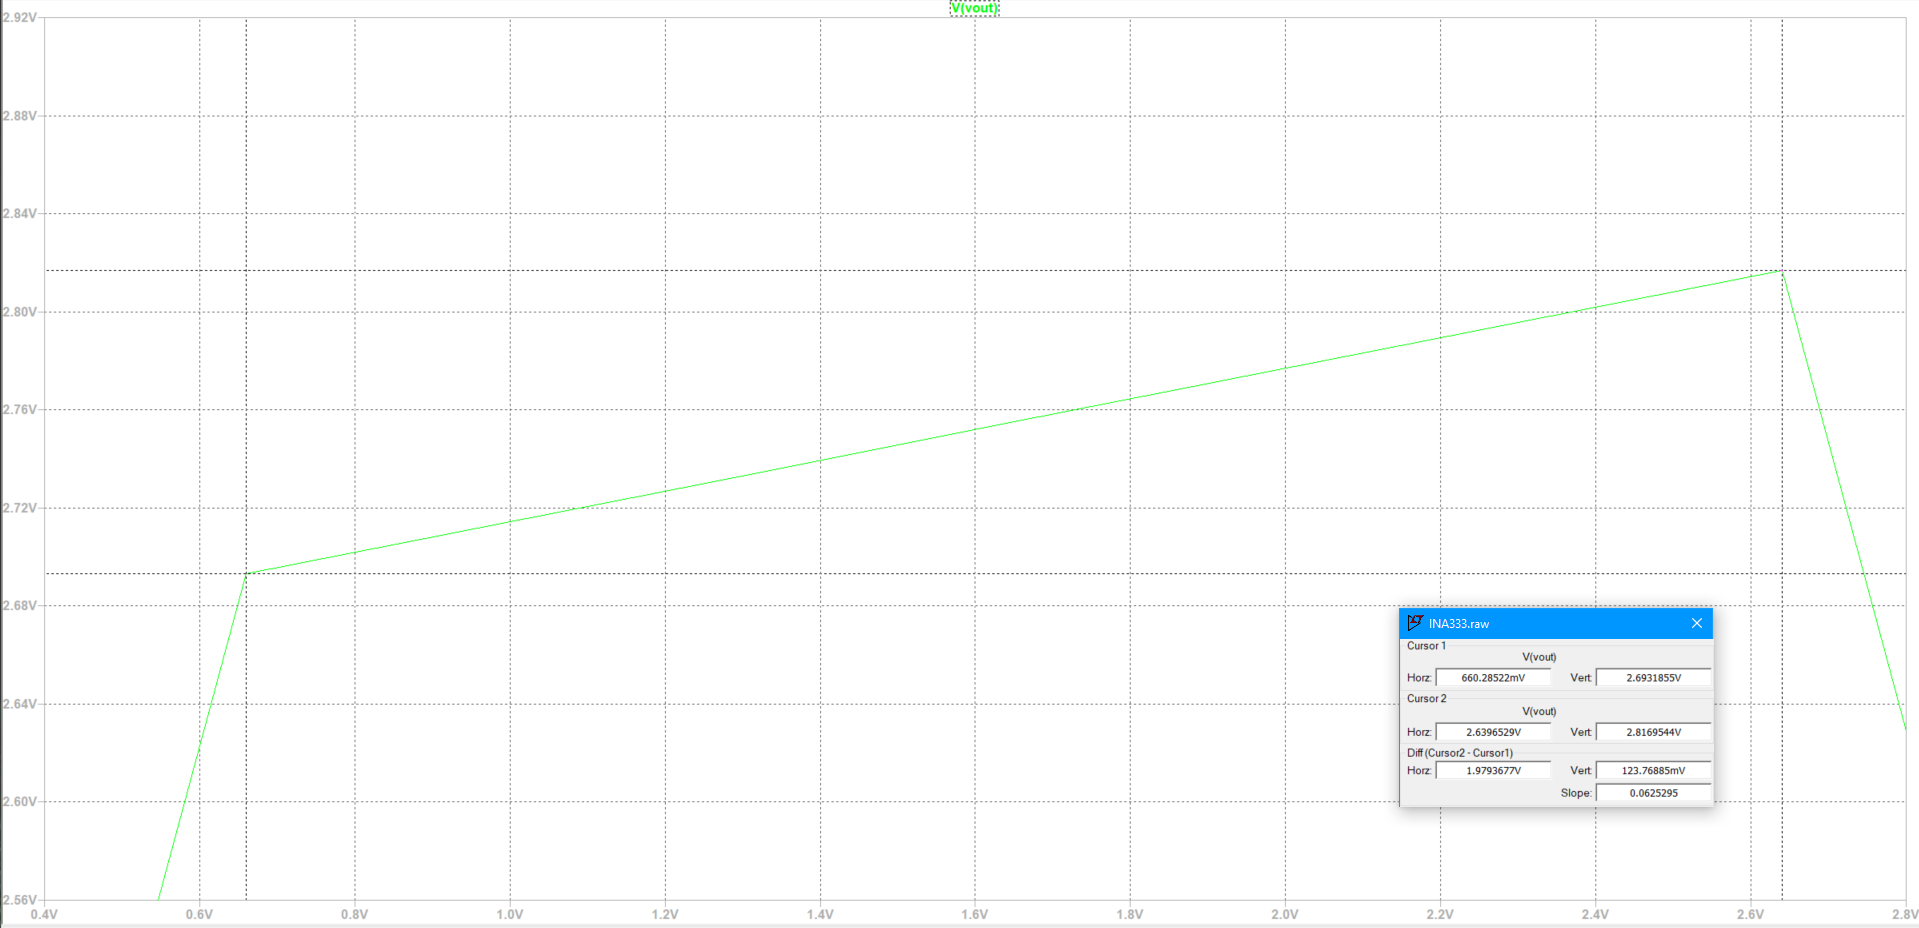
\includegraphics[width=\textwidth]{INA333_p1u_cm.png}
        \caption{Symulacja dc wejściowego napięcia wspólnego wzmacniacza pomiarowego dla $I_{meas} = 1\ \mu A$, różnica napięć $\approx 120\ mV$.}
        \label{fig:sym_INA_CM}
    \end{figure}
    \clearpage
    \begin{figure}[!ht]
        \centering
        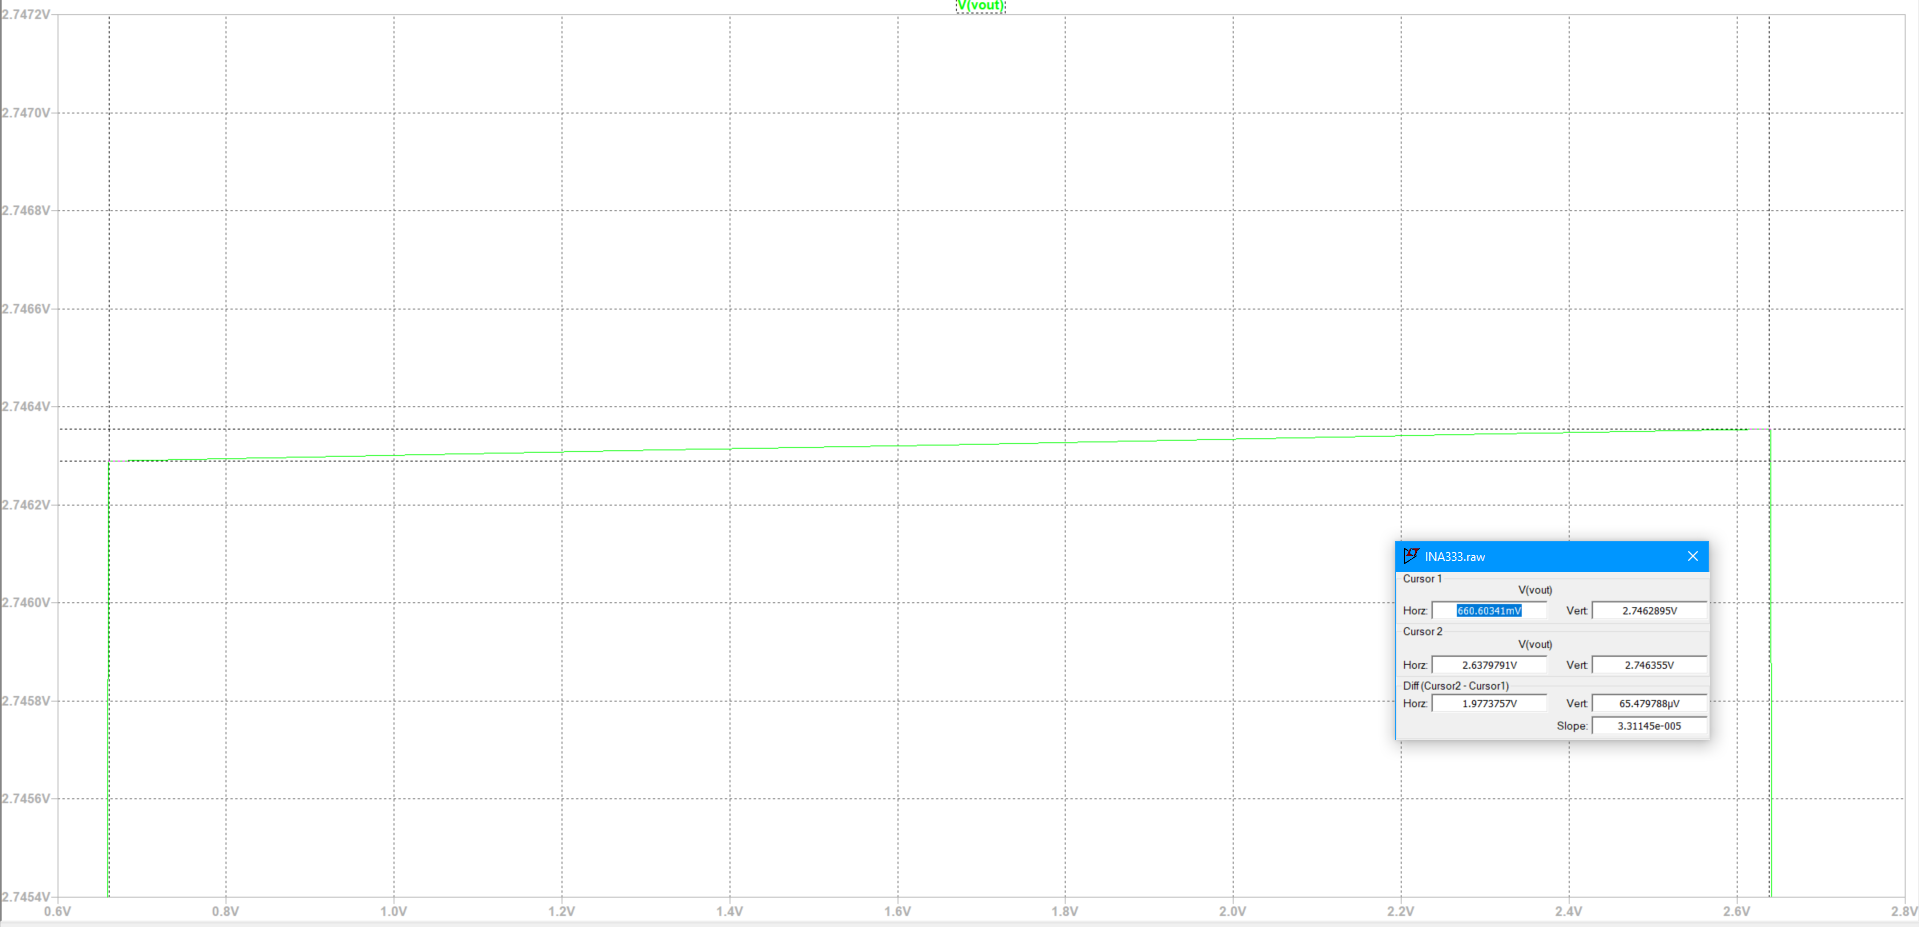
\includegraphics[width=\textwidth]{INA333_p1u_cm_follower.png}
        \caption{Symulacja dc wejściowego napięcia wspólnego wzmacniacza pomiarowego z buforowaniem $V_{REF}$ dla $I_{meas} = 1\ \mu A$, różnica napięć $\approx 65\ \mu V$.}
        \label{fig:sym_INA_CM_follower}
    \end{figure}
    \begin{figure}[!ht]
        \centering
        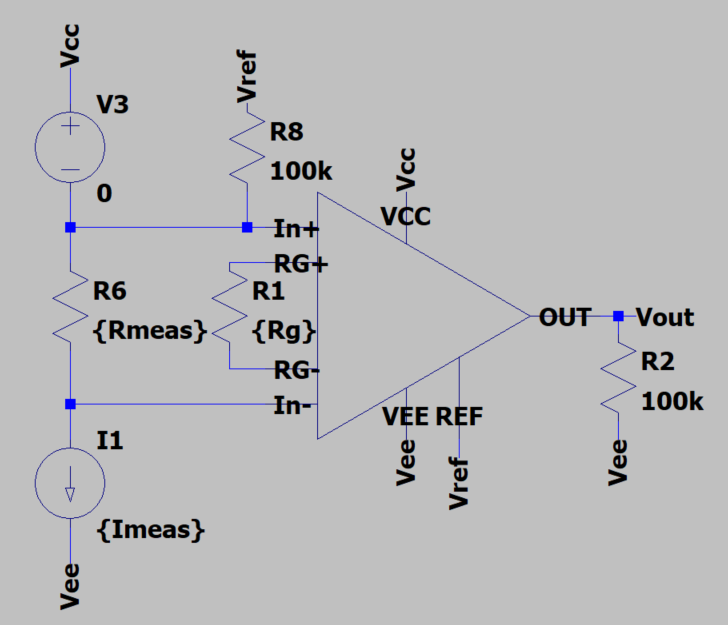
\includegraphics[width=0.7\textwidth]{INA333_cm_sim.png}
        \caption{Schemat do symulacji $V_{CM}$.}
        \label{fig:sym_CM_sch}
    \end{figure}
